% !TEX TS-program = pdflatex
% !TEX encoding = UTF-8 Unicode

% This is a simple template for a LaTeX document using the "article" class.
% See "book", "report", "letter" for other types of document.

\documentclass[8pt]{article} % use larger type; default would be 10pt

\usepackage[utf8]{inputenc} % set input encoding (not needed with XeLaTeX)
\usepackage{bchart}
\usepackage{longtable}
\usepackage{pgfgantt}
\usepackage{calendar} % Use the calendar.sty style


%%% Examples of Article customizations
% These packages are optional, depending whether you want the features they provide.
% See the LaTeX Companion or other references for full information.

\usepackage{textcomp}
%\usepackage{hyperref}

%%% PAGE DIMENSIONS
\usepackage{geometry} % to change the page dimensions
\geometry{a4paper} % or letterpaper (US) or a5paper or....
% \geometry{margin=2in} % for example, change the margins to 2 inches all round
% \geometry{landscape} % set up the page for landscape
%   read geometry.pdf for detailed page layout information

\usepackage{graphicx} % support the \includegraphics command and options

% \usepackage[parfill]{parskip} % Activate to begin paragraphs with an empty line rather than an indent

%%% PACKAGES
\usepackage{booktabs} % for much better looking tables
\usepackage{array} % for better arrays (eg matrices) in maths
\usepackage{paralist} % very flexible & customisable lists (eg. enumerate/itemize, etc.)
\usepackage{verbatim} % adds environment for commenting out blocks of text & for better verbatim
\usepackage{subfig} % make it possible to include more than one captioned figure/table in a single float
% These packages are all incorporated in the memoir class to one degree or another...

%%% HEADERS & FOOTERS
\usepackage{fancyhdr} % This should be set AFTER setting up the page geometry
\pagestyle{fancy} % options: empty , plain , fancy
\renewcommand{\headrulewidth}{0pt} % customise the layout...
\lhead{}\chead{}\rhead{}
\lfoot{}\cfoot{\thepage}\rfoot{}

%%% SECTION TITLE APPEARANCE
\usepackage{sectsty}
\allsectionsfont{\sffamily\mdseries\upshape} % (See the fntguide.pdf for font help)
% (This matches ConTeXt defaults)

%%% ToC (table of contents) APPEARANCE
\usepackage[nottoc,notlof,notlot]{tocbibind} % Put the bibliography in the ToC
\usepackage[titles,subfigure]{tocloft} % Alter the style of the Table of Contents
\renewcommand{\cftsecfont}{\rmfamily\mdseries\upshape}
\renewcommand{\cftsecpagefont}{\rmfamily\mdseries\upshape} % No bold!

%%% END Article customizations

%%% The "real" document content comes below...

\title{Management overview}
\author{\copyright Frederic Kerdraon}
%\date{} % Activate to display a given date or no date (if empty),
         % otherwise the current date is printed 

\begin{document}
\maketitle
\tableofcontents
\section{Introduction}

This document summurizes all the important informations necessary to facilitate things and remove a lot of stress. It's been put together thanks to \LaTeX. This is design to help make optimal decisions for a not so short lifetime.

Ce n'est pas parceque les choses sont difficiles que nous n'osons pas, c'est parceque nous n'osons pas qu'elles sont difficiles.
%\makebox[2\width]{hello}
\texteuro

\section{Communication and administration}
\subsection{Mummy weekly call}
\subsection{Daddy weekly call}
\subsection{Karima weekly call}

\section{Calendars}
\subsection{Yearly calendar}

\begin{calendar}{\hsize}
 
%----------------------------------------------------------------------------------------
%	BLANK DAYS BEFORE THE BEGINNING OF THE CALENDAR
%----------------------------------------------------------------------------------------

% This part is very finicky. It defines the number of blank days at the beginning of the calendar before the first of the month starts. If you need this to be more than 4 (i.e. the first starts on a Friday or Saturday in a 31 day month), then you have two options: 
% 1) You can uncomment another one or two \BlankDay's below which will make a new week (6 total) which makes the calendar too big for one page, remedy this by decreasing the size of each day by replacing 2.5cm below with a smaller number. 
% 2) Make the spill-over days start at the top left of the calendar (i.e. the calendar starts with 31 then a few days blank then 1, 2, 3, etc). The second option can be configured by uncommenting the below:

%\setcounter{calendardate}{31} % Begin the count with 31 so the top left day is 31; this can be changed to 29 or 30 as required
%\day{}{\vspace{2.5cm}} % 31 - add another line identical to this if starting at 30 or earlier

% You will need to comment out the 31 in the NUMBERED DAYS AND CALENDAR CONTENT section below for this as well as commenting out one of the \BlankDay's below. Play around with it and you will get it.

\BlankDay
\BlankDay
%\BlankDay
%\BlankDay
%\BlankDay
%\BlankDay

%----------------------------------------------------------------------------------------
%	NUMBERED DAYS AND CALENDAR CONTENT
%----------------------------------------------------------------------------------------

% These are the numbered days in the template - if there are less than 31 days simply comment out the bottom lines.

% \vspace{2.5cm} is only there to provide an even look to the calendar where each day is 2.5cm tall, it can be changed or removed to automatically adjust to the day in the week with the most content

\setcounter{calendardate}{1} % Start the date counter at 1

\day{Work}{10am Meeting with Boss \\[6pt] 12pm Meeting with Group} % 1 - Example of content
\day{}{\vspace{2.5cm}} % 2 
\day{}{\vspace{2.5cm}} % 3
\day{}{\vspace{2.5cm}} % 4
\day{}{\vspace{2.5cm}} % 5
\day{}{\vspace{2.5cm}} % 6
\day{}{\vspace{2.5cm}} % 7
\day{}{\vspace{2.5cm}} % 8
\day{}{\vspace{2.5cm}} % 9
\day{}{\vspace{2.5cm}} % 10
\day{}{\vspace{2.5cm}} % 11
\day{}{\vspace{2.5cm}} % 12
\day{}{\vspace{2.5cm}} % 13
\day{}{\vspace{2.5cm}} % 14
\day{}{\vspace{2.5cm}} % 15
\day{}{\vspace{2.5cm}} % 16
\day{}{\vspace{2.5cm}} % 17
\day{}{\vspace{2.5cm}} % 18
\day{}{\vspace{2.5cm}} % 19
\day{}{\vspace{2.5cm}} % 20 
\day{}{\vspace{2.5cm}} % 21
\day{}{\vspace{2.5cm}} % 22
\day{}{\vspace{2.5cm}} % 23
\day{}{\vspace{2.5cm}} % 24
\day{}{\vspace{2.5cm}} % 25
\day{}{\vspace{2.5cm}} % 26
\day{}{\vspace{2.5cm}} % 27
\day{}{\vspace{2.5cm}} % 28
\day{}{\vspace{2.5cm}} % 29 
\day{}{\vspace{2.5cm}} % 30 
\day{}{\vspace{2.5cm}} % 31

% Un-comment the \BlankDay below if the bottom line of the calendar is missing
%\BlankDay

% Un-comment to start counting again after 31
%\setcounter{calendardate}{1}
%\day{}{\vspace{2.5cm}} % 1
%\day{}{\vspace{2.5cm}} % 2
%\day{}{\vspace{2.5cm}} % 3

%----------------------------------------------------------------------------------------

\finishCalendar
\end{calendar}

\subsection{Weekly calendar}
\begin{calendar}{\hsize}

%----------------------------------------------------------------------------------------
%	FIRST DAY
%----------------------------------------------------------------------------------------

\day{}{\textbf{9am-5pm} \daysep Work at McDonald's} % By default all daily events are centered in the box, in order to bring them up use \vspace{2cm} after the event text; you may need to change the 2cm

%----------------------------------------------------------------------------------------
%	SECOND DAY
%----------------------------------------------------------------------------------------

\day{}{
\textbf{9am-10am} \daysep BIOSCI101 - BLT100 \\[3pt]
\textbf{10am-11am} \daysep BIOSCI 104 - LLT \\[3pt]
%\textbf{11am-12pm} \daysep No Lecture \\[3pt]
\textbf{12pm-1pm} \daysep BIOSCI105 - BLT204 \\[3pt]
%\textbf{1pm-2pm} \daysep No Lecture \\[3pt]
\textbf{2pm-5pm} \daysep BIOSCI101 Laboratory \\[3pt]
%\textbf{3pm-4pm} \daysep BIOSCI101 Laboratory \\[3pt]
%\textbf{4pm-5pm} \daysep BIOSCI101 Laboratory
} 

%----------------------------------------------------------------------------------------
%	THIRD DAY
%----------------------------------------------------------------------------------------

\day{}{ % Tuesday
\textbf{9am-10am} \daysep BIOSCI101 - BLT100 \\[3pt]
\textbf{10am-11am} \daysep BIOSCI 104 - LLT \\[3pt]
%\textbf{11am-12pm} \daysep No Lecture \\[3pt]
%\textbf{12pm-1pm} \daysep No Lecture \\[3pt]
%\textbf{1pm-2pm} \daysep No Lecture \\[3pt]
\textbf{2pm-3pm} \daysep GEO101 - HSB1 \\[3pt]
%\textbf{3pm-4pm} \daysep No Lecture \\[3pt]
%\textbf{4pm-5pm} \daysep No Lecture
} 

%----------------------------------------------------------------------------------------
%	FOURTH DAY
%----------------------------------------------------------------------------------------

\day{}{ % Wednesday
%\textbf{9am-10am} \daysep No Lecture \\[3pt]
\textbf{10am-11am} \daysep BIOSCI 104 - LLT \\[3pt]
%\textbf{11am-12pm} \daysep No Lecture \\[3pt]
\textbf{12pm-1pm} \daysep BIOSCI105 - BLT204 \\[3pt]
%\textbf{1pm-2pm} \daysep No Lecture \\[3pt]
\textbf{2pm-3pm} \daysep GEO101 - HSB1 \\[3pt]
%\textbf{3pm-4pm} \daysep No Lecture \\[3pt]
%\textbf{4pm-5pm} \daysep No Lecture
} 

%----------------------------------------------------------------------------------------
%	FIFTH DAY
%----------------------------------------------------------------------------------------

\day{}{ % Thursday
%\textbf{9am-10am} \daysep No Lecture \\[3pt]
\textbf{10am-11am} \daysep BIOSCI 104 - LLT \\[3pt]
%\textbf{11am-12pm} \daysep No Lecture \\[3pt]
%\textbf{12pm-1pm} \daysep No Lecture \\[3pt]
%\textbf{1pm-2pm} \daysep No Lecture \\[3pt]
\textbf{2pm-3pm} \daysep GEO101 - HSB1 \\[3pt]
%\textbf{3pm-4pm} \daysep No Lecture \\[3pt]
%\textbf{4pm-5pm} \daysep No Lecture
} 

%----------------------------------------------------------------------------------------
%	SIXTH DAY
%----------------------------------------------------------------------------------------

\day{}{ % Friday
\textbf{9am-10am} \daysep BIOSCI101 - BLT100 \\[3pt]
\textbf{10am-11am} \daysep BIOSCI 104 - LLT \\[3pt]
%\textbf{11am-12pm} \daysep No Lecture \\[3pt]
\textbf{12pm-1pm} \daysep BIOSCI105 - BLT204 \\[3pt]
%\textbf{1pm-2pm} \daysep No Lecture \\[3pt]
%\textbf{2pm-3pm} \daysep No Lecture \\[3pt]
\textbf{3pm-4pm} \daysep GEO101 Tutorial \\ Room A \\[3pt]
%\textbf{4pm-5pm} \daysep No Lecture
} 

%----------------------------------------------------------------------------------------
%	SEVENTH DAY
%----------------------------------------------------------------------------------------

\day{}{} % Saturday

%----------------------------------------------------------------------------------------
 
\finishCalendar
\end{calendar}


\section{Crew}
Zaz - Carte/VHF/GPS/Route
Yann - Matossage/Cuisine/Pharmacie
Christophe - Voile/Theatre/Chant/Motor
Lionel - Barre/Second/Route
Fred - Guitar/Skipper/Funding/Project management/Resources


\section{Receipes}

4e per person - 1/2h  + 10mns/person\\
Rate = cost per person*time \\
Number of times done\\
Time to prepare\\
Tools necessary\\
Energy cost\\

Salade de printemps\\
Crepes\\
Boeauf au four\\
Spagettis a la vietnamienne\\
Poulet au curry\\

\section{References}
\subsection{books}
\subsection{links}

Moitessier - saloon\\
Nietzche - desk\\
Dali - desk\\
Music - desk\\
Bible - room\\
Coran - room\\
Sidarta - room\\
Jack Kerouac - desk\\
Moliere Dom Juan - desk\\

%http://en.wikibooks.org/wiki/LaTeX/Mathematics
%\url{http://www.wikibooks.org}
%\href{http://www.wikibooks.org}{Wikibooks home}

%PERT Diagram : http://fr.wikipedia.org/wiki/R%C3%A9seau_PERT
%Burn down chart : http://en.wikipedia.org/wiki/Scrum_%28development%29
%Theory of constraints : http://en.wikipedia.org/wiki/Theory_of_constraints
%Leverage points : http://en.wikipedia.org/wiki/Twelve_leverage_points
%Linear programing : http://en.wikipedia.org/wiki/Linear_programming
%Markov chains :(Information theory) http://en.wikipedia.org/wiki/Markov_chain
%Information : http://en.wikipedia.org/wiki/Information_entropy
%http://makerplane.org/?page_id=168
%http://en.wikipedia.org/wiki/Wikispeed

%http://en.wikipedia.org/wiki/Three_stratum_theory
%http://en.wikipedia.org/wiki/M%C3%B6bius_transformation
%http://en.wikipedia.org/wiki/Hypergeometric_function
%http://en.wikipedia.org/wiki/Laguerre_polynomial#Generalized_Laguerre_polynomials
%http://en.wikipedia.org/wiki/Schr%C3%B6dinger_equation
%http://en.wikipedia.org/wiki/Langevin_equation
%http://en.wikipedia.org/wiki/Brownian_motion
%http://en.wikipedia.org/wiki/General_relativity


\section{Tasks}

Weight, deadline, ROI

Poster la bouee en U
Reparer le feu de retournement
Reparer la traine
Installer une ligne sur la canne
Nettoyer le pont
Graisser la barre
Refermer la trappe
Faire la vaisselle
Nettoyer les banettes
Nettoyer les inox
Masque? CMB?
Verifier le mouillage
Reparer la manette de vitesse
Scotcher les haubans - done
Installer le son
Plonger pour carenner
Ameliorer la connexion batterie
Fixer le 12v sur le tableau
Changer le mode du rechaud
Reparer la voile
Rincer le spi et tous les bouts
Ajuster les amarres
Installer le GPS
Changer les lampes
Nettoyer la glaciere
Reparer le stick
Vernis bois clair
Recuperer de la garcette
Mettre un paillasson
Recoler les lettres Jeanneau
Recoller le morceau de bois interieur
Essence a briquet
Piles R6
Fer a souder
Ranger la cave
Regonfler velo
Carenner le bateau


Sac
Scotch
Testeur batterie
w30
caisse a outils
lingettes
brosse
eponge
essuie tout
scratch
lampes
brosse metallique
barbecue
tuyau
vernis a bois
karcher

\section{Investments}

\section{Skills}

rating - experience (years) - 

Project management\\
Finance\\
Risk management\\
Organisation\\
Communication\\
International negociations\\
Career development\\
Sponsorship\\
Information technology\\
Design\\
Architecture\\
Plastic arts\\
Sports\\
Navigation\\
Piloting\\
Driving\\
Philosophy\\
Guitar\\
Religion\\
Horse riding\\
Dessin\\
Maths et physics\\
Guitar\\
Football\\
Gardening\\
Arts\\
Social behaviour\\
Running\\
Fashion\\
Religion\\
Horse riding\\


\section{Rate}

\begin{bchart}[min=0,max=10000,step=5000,unit=m\textsuperscript{2}]
  \bcbar[label=Daily]{400}
  \bcbar[label=Weekly]{1900}
  \bcbar[label=Monthly]{7600}
  \bcbar[label=3 Months]{10000}
  \smallskip
  \medskip
  \bigskip
\end{bchart}

\section{Health}
Cigarettes\\
Beers\\
Joints\\
Sleep\\
Internet\\
Whisky\\
Wine\\


\section{Loss}
Julbo - 80e - Etienne
Parre batte - 40e - Fred
Lampe torche - 50e - Christophe
Traine - 25e - Ronan
Sac spi - 30e - Zaz
Interface Elec - 17e - Etienne

\section{Checklists}
\subsection{Daily Morning}
	
\subsection{2 weeks trip}			
\begin{calendar}{\hsize}

\setcounter{calendardate}{4} % Date on which the calendar starts - note that you have to account for blank days

%----------------------------------------------------------------------------------------
%	FIRST DAY
%----------------------------------------------------------------------------------------

\BlankDay 

%----------------------------------------------------------------------------------------
%	SECOND DAY
%----------------------------------------------------------------------------------------

\BlankDay 

%----------------------------------------------------------------------------------------
%	THIRD DAY
%----------------------------------------------------------------------------------------

\BlankDay 

%----------------------------------------------------------------------------------------
%	FOURTH DAY
%----------------------------------------------------------------------------------------

\day{In Transit}{
\textbf{Depart} (PHL) @ 18:10 EDT\\
US Airways \# 740\\
US Airways record locator: EPYTWQ\\
Airline ticket number(s): 0377186181588-589
}

%----------------------------------------------------------------------------------------
%	FIFTH DAY
%----------------------------------------------------------------------------------------

\day{Madrid}{
\textbf{Arrive} (MAD) @ 07:45 CEST\\\daysep
Hotel Senator Gran V\'ia\\
Calle Gran V\'ia, 21\\
28013 (Centro) MADRID\\
+34 915 31 41 51\\
Reservation code: 080131-98638\\
Cancellation code: 9860291\\\daysep
Palacio Real\\
Plaza Mayor\\
Reina Sof\'ia National Museum
}

%----------------------------------------------------------------------------------------
%	SIXTH DAY
%----------------------------------------------------------------------------------------

\day{Toledo (Day Trip)}{
Cathedral\\
Sinagoga del Transito\\
Palace Alcazar\\
Sinagoga del Santa Maria la Blanca
}

%----------------------------------------------------------------------------------------
%	SEVENTH DAY
%----------------------------------------------------------------------------------------

\day{Madrid}{
Real Academic de Bellas Artes\\Templo de Debod\\Museo del Prado\\\daysep
\textbf{Depart} Madrid @ 22:45 on SNCF 332
}

%----------------------------------------------------------------------------------------
%	EIGHTH DAY
%----------------------------------------------------------------------------------------

\day{Lisbon}{
\textbf{Arrive} in Lisbon @ 08:00\\\daysep
Hotel Real Pal\'acio\\
Rua Tom\'as Ribeiro 115\\\ \\
Elevador de Santa Justa\\
Solar do Vinho do Porto\\
Castelo de S\~ao Jorge\\Mosteiro do Geron\'imos\\Torre de Bel\'em
}

%----------------------------------------------------------------------------------------
%	NINTH DAY
%----------------------------------------------------------------------------------------

\day{Estoril}{
\textbf{Arrive} in Estoril\\\daysep
Hotel Alvorada\\
Rua de Lisboa, 3\\\daysep
OptMAS Workshop?\\
}

%----------------------------------------------------------------------------------------
%	TENTH DAY
%----------------------------------------------------------------------------------------

\day{Estoril}{
DCR Workshop
}

%----------------------------------------------------------------------------------------
%	ELEVENTH DAY
%----------------------------------------------------------------------------------------

\day{Estoril}{
FIPA Meeting 11:10--12:10\\
Poster Session w/``Drinks and Snacks'' 15:00--16:00
}

%----------------------------------------------------------------------------------------
%	TWELFTH DAY
%----------------------------------------------------------------------------------------

\day{Estoril}{ 
AAMAS Demos\\
Conference Banquet @ 18:30
}

%----------------------------------------------------------------------------------------
%	THIRTEENTH DAY
%----------------------------------------------------------------------------------------

\day{Estoril}{
\textbf{Depart} (LIS) @ 10:35 WEST\\
US Airways \#739\\
\textbf{Arrive} (PHL) @ 13:25 EST
}

%----------------------------------------------------------------------------------------
%	FOURTEENTH DAY
%----------------------------------------------------------------------------------------

\BlankDay

%----------------------------------------------------------------------------------------
% More days can be added to give the calendar a third or fourth week
%----------------------------------------------------------------------------------------

\finishCalendar
\end{calendar}

\subsection{Week-end trip}			
\subsection{Sailing trip}			
\subsection{Complete relocation}			
	Packaging and posting			\\
	Flight			\\
	Last day			\\
	Move preparation			\\
	Boat yearly maintenance			\\
\subsection{Two weeks trip}
coupe ongle\\
brosse a cheveux\\
brosse a dent\\
dentifrice\\
cles de la maison\\
cles de la destination\\
cadeau hotes\\
tongues\\
polaire\\
carte destination\\
bouquin pour le trajet\\
gel douche/shampoing\\
appareil photo\\
telephone\\
billets de train/avion\\
sac a dos\\
manteau ou veste pour le temps\\
check meteo\\
sun glasses\\
solar cream\\
laptop\\
portfolio\\
access cards\\
underwear\\
tee shirts\\
water\\
planning\\
paper phone numbers\\
casque musique\\
videos\\

\subsection{Week-end trip}
sac de couchage\\
tentes\\
2 underwares\\
100 euro\\
some music\\
grosses chaussettes\\
marteau\\

\subsection{Sailing trip}
Carte,GPS,VHF,Lampe,meteo,maree\\

\section{Management}
\subsection{Ludo}
	Toutes les 2 semaines passer a recou (60euro+binouzes)\\
\subsection{Karima}
	Me laisser aider sur la methodo et l'orga\\
	Me laisser un acces a distance\\
	Si le systeme marche, ca ne sera que du bonheur pour toi\\
	J'ai une vie personelle\\
\subsection{Aymeric}
	Fermer sa gueule\\
\subsection{Francois}
	Expliquer volant Alfa\\
\subsection{Nicolas}
	Rester dormir a la maison avec Antoine\\
	Venir avec les filles pour le shopping rue de siam\\
\subsection{Jean Alexandre}
	Be around\\
\subsection{Zaz}
	Me garde ma voiture, \\
	Vient me chercher toutes les semaines a la gare\\
	Poker a la maison le vendredi soir\\
\subsection{Rico}
	Entretien Plijadur\\
	Amener Pascal et Daniel faire du bateau\\
	Juliette et Antoine\\
	Ludo\\
	Arreter ses petites reflexion sur moi\\
\subsection{Yann}
	S'occuper des plantes a Plougastel\\
\subsection{Maeva}
	Amener son cheval\\
	Parler a Elise\\
\subsection{Maman}
	Menage tous les jeudi\\
\subsection{Elise}
	Cf Fifty shades of Fred\\
	Ne rien raconter de ce que l'on fait\\
	Faire les ajustements sur la robe !\\
\subsection{Lionel}
	Faire le necessaire pour Plijadur\\
\subsection{Flo}
	Passer a la maison de temps en temps\\
\subsection{Nicole}
	Me vendre l'appartement \\
\subsection{Laurent}
	Garder mon alfa\\
	Venir avec moi a sein\\
\subsection{Julien}
	M'apprendre Murex\\
	
\subsection{Christian}

Il faut juste apprendre a partager pour faire des economies et etre heureux\\

Books			\\
	
\subsection{Guillaume}
	Faire les commentaires sur mes morceaux
		
\subsection{Phil}
	Me garder une place au chaud a Hong Kong

\subsection{Wing}
	Me garder mes potes de hong kong

\section{Friends origins}
Algerie			\\
Maroc - Fouad			\\
France			\\
Italie	- Armando		\\
Chine			\\
Slovaquie	- Miro		\\
Taiwan			\\
Thailand	- Thip, Anita	\\
United states			\\
Spain		- Jorge	\\
Greece\\	
England			\\
Scotland			\\
Wales			\\
New zealand	- Brett		\\
South Africa	- Jason		\\
Australia			\\
Russia			\\
Indonesia			\\
Zimbaboue			\\
Cameroun	- Francky		\\
Vietnam			\\
Columbia			\\

\section{Diplomas}
Brevet des colleges			\\
Baccalaureat			\\
Ingenieur			\\
Permis nav			\\
Brevet ulm			\\
Brevet pilote			\\

\section{Mis behaviour}
Fine for cannabis posetion festival			\\
Fine for cannabis posetion liberte			\\
Taxes fines			\\
Speed fines			\\
 
\section{Plijadur Credits}

Plijadur, la vie a la dure... \\
Jean Alexandre Binoche - 4\\
Li Mai - 4\\
Mag - 1			\\
Rico - 10			\\
Sonia	- 4		\\
Wing	- 2		\\
Zaz	- 5		\\
Lionel - 2			\\
Yann	- 1		\\
Canet	- 3		\\
Maeva	- 3		\\
Armelle	- 3		\\

\section{Curriculum vitae}

\section{Climate camp}
toilettes seche			\\
tent			\\
eolienne			\\
solar panel			\\
battery			\\
metal "malle"			\\
chauffe eau solaire			\\
poele			\\
composteur			\\
abri de jardin			\\
			
\section{Culture}
Bamboos - Papyrus			\\
Cannabis			\\
Strawberries			\\
Salads			\\
Avoine			\\
Tomatoes			\\
Thym			\\
Plasil			\\
Laurier			\\
Rosier			\\
Kalankoe			\\
Ficus			\\
Bananier			\\
Citrons			\\
Pommes de terre			\\
Kiwis			\\

\section{Finance}

\subsection{Transactions1}
{\footnotesize
\begin{longtable}{|c|c|c|}
\hline
\multicolumn{3}{|c|}{Liabilities} \\
\hline
07/11 & PRLV   PREDICA GARANTIE DECES & 4,87 \\
\hline
07/11 & **COTISATION CS OPTION 2 & 6,00 \\
\hline
06/11 & RET DAB COURBEVOIE     05 11 12 & 80,00 \\
\hline
06/11 & RET DAB BREST          03 11 12 & 40,00 \\
\hline
05/11 & CARTE SNCF             05/11/12 & 185,60 \\
\hline
05/11 & CARTE TAXI PAULO       03/11/12 & 50,00 \\
\hline
05/11 & CARTE CASINO 24 PORTE  04/11/12 & 18,60 \\
\hline
05/11 & CARTE SUPERETTE RECOUV 03/11/12 & 10,80 \\
\hline
05/11 & PRLV   DOSSIER FAMILIAL & 9,90 \\
\hline
05/11 & ** COTIS.SERVICE GAEL & 1,13 \\
\hline
02/11 & CARTE WP EASYROOMMATE  01/11/12 & 21,90 \\
\hline
02/11 & CARTE RATP             01/11/12 & 1,70 \\
\hline
02/11 & VIR.MONFORT NICOLE & 486,00 \\
\hline
29/10 & PRLV   ASS PACIFICA  05973356907 & 486,00 \\
\hline
26/10 & RET DAB BREST          25 10 12 & 13,09 \\
\hline
26/10 & CARTE LA POSTE 299240  25/10/12 & 40,00 \\
\hline
26/10 & CARTE SUPERETTE RECOUV 25/10/12 & 23,00 \\
\hline
25/10 & CARTE CASINO 24 PORTE  24/10/12 & 15,80 \\
\hline
24/10 & CARTE REL.TOTAL 59934  23/10/12 & 10,40 \\
\hline
24/10 & CARTE LA POSTE 299240  23/10/12 & 79,40 \\
\hline
24/10 & PRLV 332801   SFR MOBILE & 23,00 \\
\hline
23/10 & RET DAB BREST          21 10 12 & 51,74 \\
\hline
22/10 & CARTE CASINO 24 PORTE  19/10/12 & 60,00 \\
\hline
19/10 & PRLV   SUPPLETIS & 15,60 \\
\hline
18/10 & RET DAB BREST          17 10 12 & 20,00 \\
\hline
16/10 & RET DAB 06321 LE RELEC 14 10 12 & 60,00 \\
\hline
16/10 & CARTE CUPID.COM 448005 13/10/12 & 80,00 \\
\hline
16/10 & CARTE SUPERETTE RECOUV 15/10/12 & 45,99 \\
\hline
15/10 & CARTE TABAC PR DIDOU   12/10/12 & 31,40 \\
\hline
15/10 & RET DAB BREST CENTRE   13 10 12 & 66,00 \\
\hline
15/10 & CARTE SUPERETTE RECOUV 12/10/12 & 60,00 \\
\hline
15/10 & CARTE SUPERETTE RECOUV 14/10/12 & 15,70 \\
\hline
15/10 & PRLV   ASS PACIFICA  06019130907 & 12,30 \\
\hline
12/10 & RET DAB MARIGNANE CEDE 11 10 12 & 67,15 \\
\hline
12/10 & CARTE BIBUS            11/10/12 & 40,00 \\
\hline
11/10 & RET DAB LCL MARSEILLE  10 10 12 & 2,70 \\
\hline
10/10 & RET DAB MARSEILLE CAST 09 10 12 & 40,00 \\
\hline
10/10 & CARTE LINSOLITE        09/10/12 & 40,00 \\
\hline
10/10 & PRLV ECH PRET A CONSOMMER & 27,50 \\
\hline
10/10 & PRLV ECH PRET A CONSOMMER & 383,59 \\
\hline
09/10 & CARTE SFR ESPACE       08/10/12 & 146,90 \\
\hline
09/10 & RET DAB MARIGNANE CEDE 06 10 12 & 64,80 \\
\hline
09/10 & RET DAB BREST          06 10 12 & 40,00 \\
\hline
09/10 & RET DAB MARSEILLE      08 10 12 & 40,00 \\
\hline
09/10 & PRLV 001007   ELECTRICITE DE FRA & 40,00 \\
\hline
09/10 & PRLV   PREDICA GARANTIE DECES & 65,00 \\
\hline
08/10 & CARTE SARL NISSANA     07/10/12 & 4,87 \\
\hline
08/10 & CARTE MARCHE PLUS      06/10/12 & 29,40 \\
\hline
08/10 & CARTE SUPERETTE RECOUV 05/10/12 & 14,93 \\
\hline
08/10 & CARTE CASINO 24 PORTE  06/10/12 & 14,60 \\
\hline
08/10 & CARTE VOL24.FR         05/10/12 & 12,00 \\
\hline
08/10 & **COTISATION CS OPTION 2 & 10,78 \\
\hline
05/10 & CARTE RYANAIR          03/10/12 & 6,00 \\
\hline
05/10 & CARTE VOL24.FR         03/10/12 & 88,40 \\
\hline
05/10 & CARTE SUPERETTE RECOUV 04/10/12 & 19,73 \\
\hline
04/10 & CARTE SUPERETTE RECOUV 03/10/12 & 12,70 \\
\hline
03/10 & RET DAB 06321 LE RELEC 02 10 12 & 9,10 \\
\hline
03/10 & CARTE SUPERETTE RECOUV 02/10/12 & 80,00 \\
\hline
03/10 & CARTE MC DONALD'S      02/10/12 & 15,20 \\
\hline
03/10 & CARTE SUPER U          02/10/12 & 11,30 \\
\hline
02/10 & CARTE SNCF             01/10/12 & 51,90 \\
\hline
02/10 & RET DAB PARIS          01 10 12 & 79,60 \\
\hline
02/10 & CARTE SUSHI FOLIES     01/10/12 & 40,00 \\
\hline
02/10 & CARTE EFFIA CSIONS     01/10/12 & 13,50 \\
\hline
02/10 & ** COTIS.SERVICE GAEL & 7,30 \\
\hline
01/10 & CARTE SNCF INTERNET    30/09/12 & 1,13 \\
\hline
01/10 & CARTE SUPERETTE RECOUV 28/09/12 & 91,00 \\
\hline
01/10 & CARTE SUPERETTE RECOUV 30/09/12 & 35,20 \\
\hline
01/10 & VIR.MONFORT NICOLE & 19,90 \\
\hline
28/09 & PRLV   ASS PACIFICA  05973356907 & 486,00 \\
\hline
27/09 & CARTE SUPERETTE RECOUV 26/09/12 & 13,13 \\
\hline
27/09 & VIR    CAPGEMINI TECHNOLOGY SER & 43,90 \\
\hline
26/09 & RET DAB SNCF MONTPARNA 25 09 12 & 60,00 \\
\hline
26/09 & CARTE EFFIA CSIONS     25/09/12 & 7,30 \\
\hline
25/09 & CARTE SNCF INTERNET    24/09/12 & 144,00 \\
\hline
24/09 & CARTE BAR TAB LE PACHA 21/09/12 & 62,00 \\
\hline
24/09 & RET DAB ST MARC BREST  22 09 12 & 60,00 \\
\hline
24/09 & CARTE SUPERETTE RECOUV 21/09/12 & 14,60 \\
\hline
24/09 & CARTE COUP'HOM         22/09/12 & 12,00 \\
\hline
24/09 & PRLV 332801   SFR MOBILE & 55,22 \\
\hline
21/09 & CARTE SUPERETTE RECOUV 20/09/12 & 14,60 \\
\hline
19/09 & RET DAB BREST          18 09 12 & 60,00 \\
\hline
19/09 & PRLV   SUPPLETIS & 20,00 \\
\hline
18/09 & CARTE SUPERETTE RECOUV 17/09/12 & 14,60 \\
\hline
17/09 & CARTE CUPID.COM 448005 13/09/12 & 45,99 \\
\hline
17/09 & CARTE SUPERETTE RECOUV 14/09/12 & 14,60 \\
\hline
17/09 & CARTE SUPERETTE RECOUV 16/09/12 & 14,60 \\
\hline
17/09 & CARTE CASINO 24 PORTE  14/09/12 & 6,60 \\
\hline
17/09 & PRLV   ASS PACIFICA  06019130907 & 68,68 \\
\hline
14/09 & CARTE SUPERETTE RECOUV 13/09/12 & 14,60 \\
\hline
13/09 & RET DAB BREST          12 09 12 & 50,00 \\
\hline
13/09 & CARTE SUPERETTE RECOUV 12/09/12 & 23,30 \\
\hline
12/09 & CARTE TABAC PR DIDOU   11/09/12 & 23,30 \\
\hline
12/09 & CARTE CASINO 24 PORTE  11/09/12 & 62,00 \\
\hline
12/09 & ** FRAIS ATD & 2,80 \\
\hline
12/09 & TVA /FRAIS & 6,44 \\
\hline
11/09 & ATD N 71775 & 1,26 \\
\hline
11/09 & VIR    C.P.A.M. FINISTERE & 77,00 \\
\hline
10/09 & CARTE CENTRE LECLERC   08/09/12 & 121,13 \\
\hline
10/09 & CARTE SUPERETTE RECOUV 07/09/12 & 11,10 \\
\hline
10/09 & CARTE SUPERETTE RECOUV 07/09/12 & 9,10 \\
\hline
10/09 & PRLV ECH PRET A CONSOMMER & 383,59 \\
\hline
10/09 & PRLV ECH PRET A CONSOMMER & 146,90 \\
\hline
10/09 & 001007 ELECTRICITE DE FRANCE & 65,00 \\
\hline
10/09 & **COTISATION CS OPTION 2 & 6,00 \\
\hline
07/09 & PRLV   PREDICA GARANTIE DECES & 4,87 \\
\hline
04/09 & ** COTIS.SERVICE GAEL & 1,13 \\
\hline
03/09 & RET DAB 06309 BREST ST 01 09 12 & 60,00 \\
\hline
03/09 & CARTE SM LES JACOBINS  01/09/12 & 39,98 \\
\hline
03/09 & CARTE SUPERETTE RECOUV 31/08/12 & 12,80 \\
\hline
01/09 & VIR.MONFORT NICOLE & 486,00 \\
\hline
30/08 & CARTE SUPERETTE RECOUV 29/08/12 & 11,00 \\
\hline
29/08 & CARTE SNC  LA PRESQU'  28/08/12 & 11,00 \\
\hline
29/08 & CARTE SUPERETTE RECOUV 28/08/12 & 62,00 \\
\hline
28/08 & CARTE REL.TOTAL 59934  27/08/12 & 11,90 \\
\hline
28/08 & RET DAB BREST          25 08 12 & 84,79 \\
\hline
28/08 & CARTE SUPERETTE RECOUV 27/08/12 & 60,00 \\
\hline
28/08 & PRLV   ASS PACIFICA  05973356907 & 14,60 \\
\hline
28/08 & **COTIS CARTE DOUBLE ACTIO & 12,37 \\
\hline
27/08 & RET DAB BREST LA FREGA 24 08 12 & 77,65 \\
\hline
27/08 & CARTE L AMIRAL NE      25/08/12 & 60,00 \\
\hline
24/08 & 332801 SFR MOBILE & 36,00 \\
\hline
23/08 & CARTE LAVAGE AUTO      22/08/12 & 55,20 \\
\hline
23/08 & CARTE SUPERETTE RECOUV 22/08/12 & 10,00 \\
\hline
21/08 & CARTE SUPERETTE RECOUV 20/08/12 & 13,10 \\
\hline
20/08 & CARTE FENDER TEX MEX   19/08/12 & 42,50 \\
\hline
17/08 & CARTE CARREFOUR BREST  16/08/12 & 28,15 \\
\hline
16/08 & CARTE CUPID.COM 448005 14/08/12 & 107,30 \\
\hline
16/08 & RET DAB BREST LA FREGA 15 08 12 & 45,99 \\
\hline
16/08 & CARTE IKEA             15/08/12 & 40,00 \\
\hline
16/08 & CARTE LE PENALTY       14/08/12 & 70,00 \\
\hline
16/08 & CARTE L'ARENA          14/08/12 & 62,00 \\
\hline
16/08 & PRLV   ASS PACIFICA  06019130907 & 4,60 \\
\hline
14/08 & RET DAB SPAR OUESSANT  12 08 12 & 68,68 \\
\hline
14/08 & CARTE L'ARENA          13/08/12 & 50,00 \\
\hline
13/08 & RET DAB BREST          10 08 12 & 10,60 \\
\hline
13/08 & CARTE LA POSTE 290190  10/08/12 & 50,00 \\
\hline
13/08 & CARTE DECATHLON 0032   10/08/12 & 23,00 \\
\hline
13/08 & RET DAB BREST          10 08 12 & 117,90 \\
\hline
13/08 & CARTE SUPERETTE RECOUV 10/08/12 & 40,00 \\
\hline
10/08 & PRLV ECH PRET A CONSOMMER & 7,20 \\
\hline
10/08 & PRLV ECH PRET A CONSOMMER & 383,59 \\
\hline
09/08 & 001007 ELECTRICITE DE FRANCE & 146,90 \\
\hline
08/08 & CARTE TOUR DU MONDE    07/08/12 & 65,00 \\
\hline
07/08 & CARTE REL.TOTAL 59934  06/08/12 & 36,00 \\
\hline
07/08 & RET DAB BREST          06 08 12 & 78,60 \\
\hline
07/08 & CARTE SARL LE BARS     06/08/12 & 40,00 \\
\hline
07/08 & PRLV   PREDICA GARANTIE DECES & 16,60 \\
\hline
07/08 & **COTISATION CS OPTION 2 & 4,87 \\
\hline
06/08 & CARTE SCUBALAND        03/08/12 & 6,00 \\
\hline
06/08 & CARTE LECLERC DB DIS   04/08/12 & 115,00 \\
\hline
06/08 & CARTE DECATHLON 0032   03/08/12 & 29,47 \\
\hline
06/08 & CARTE FENDER TEX MEX   04/08/12 & 22,95 \\
\hline
06/08 & CARTE AEROPORT PARKIN  03/08/12 & 15,90 \\
\hline
06/08 & 332801 SFR & 2,40 \\
\hline
04/08 & RET DAB FESTIVAL DU BOUT DU & 50,55 \\
\hline
02/08 & CARTE TABAC PR DIDOU   01/08/12 & 60,00 \\
\hline
02/08 & RET DAB BREST LA FREGA 01 08 12 & 62,00 \\
\hline
02/08 & CARTE CASINO 24 PORTE  01/08/12 & 60,00 \\
\hline
02/08 & CARTE LE LONGCHAMP     01/08/12 & 8,00 \\
\hline
02/08 & ** COTIS.SERVICE GAEL & 7,70 \\
\hline
01/08 & VIR.MONFORT NICOLE & 1,13 \\
\hline
31/07 & RET DAB BREST          28 07 12 & 486,00 \\
\hline
\end{longtable}

}
\subsection{Transactions2}
{\footnotesize
\begin{longtable}{|c|c|c|}
\hline
\multicolumn{3}{|c|}{Liabilities} \\
\hline
07/01 & RETRAIT AU DISTRIBUTEUR & 60,00 \\
\hline
07/01 & RETRAIT AU DISTRIBUTEUR & 40,00 \\
\hline
07/01 & PAIEMENT PAR CARTE & 24,60 \\
\hline
07/01 & PAIEMENT PAR CARTE & 44,92 \\
\hline
07/01 & PAIEMENT PAR CARTE & 19,80 \\
\hline
07/01 & PAIEMENT PAR CARTE & 150,00 \\
\hline
05/01 & PRELEVEMENT & 4,87 \\
\hline
04/01 & PAIEMENT PAR CARTE & 11,07 \\
\hline
03/01 & RETRAIT AU DISTRIBUTEUR & 100,00 \\
\hline
03/01 & PAIEMENT PAR CARTE & 34,00 \\
\hline
03/01 & PAIEMENT PAR CARTE & 50,00 \\
\hline
02/01 & COTISATION & 6,00 \\
\hline
02/01 & RETRAIT AU DISTRIBUTEUR & 60,00 \\
\hline
02/01 & PAIEMENT PAR CARTE & 21,30 \\
\hline
02/01 & PAIEMENT PAR CARTE & 28,10 \\
\hline
02/01 & PAIEMENT PAR CARTE & 84,10 \\
\hline
02/01 & PAIEMENT PAR CARTE & 83,89 \\
\hline
02/01 & PAIEMENT PAR CARTE & 35,40 \\
\hline
02/01 & VIREMENT EMIS & 486,00 \\
\hline
31/12 & RETRAIT AU DISTRIBUTEUR & 60,00 \\
\hline
31/12 & PAIEMENT PAR CARTE & 40,47 \\
\hline
31/12 & PAIEMENT PAR CARTE & 9,20 \\
\hline
28/12 & PRELEVEMENT & 65,10 \\
\hline
28/12 & PRELEVEMENT & 13,09 \\
\hline
28/12 & VIREMENT EN VOTRE FAVEUR & 13,09 \\
\hline
27/12 & PAIEMENT PAR CARTE & 132,05 \\
\hline
26/12 & RETRAIT AU DISTRIBUTEUR & 80,00 \\
\hline
26/12 & RETRAIT AU DISTRIBUTEUR & 40,00 \\
\hline
26/12 & PAIEMENT PAR CARTE & 26,90 \\
\hline
26/12 & PAIEMENT PAR CARTE & 150,00 \\
\hline
26/12 & PAIEMENT PAR CARTE & 19,99 \\
\hline
26/12 & PAIEMENT PAR CARTE & 54,80 \\
\hline
26/12 & PAIEMENT PAR CARTE & 74,95 \\
\hline
26/12 & PAIEMENT PAR CARTE & 26,90 \\
\hline
26/12 & PAIEMENT PAR CARTE & 29,00 \\
\hline
24/12 & PRELEVEMENT & 65,00 \\
\hline
24/12 & PAIEMENT PAR CARTE & 126,00 \\
\hline
24/12 & PAIEMENT PAR CARTE & 39,60 \\
\hline
24/12 & PAIEMENT PAR CARTE & 111,50 \\
\hline
24/12 & PAIEMENT PAR CARTE & 230,00 \\
\hline
24/12 & PAIEMENT PAR CARTE & 49,15 \\
\hline
24/12 & PAIEMENT PAR CARTE & 15,00 \\
\hline
24/12 & PAIEMENT PAR CARTE & 31,00 \\
\hline
21/12 & RETRAIT AU DISTRIBUTEUR & 60,00 \\
\hline
21/12 & PAIEMENT PAR CARTE & 21,30 \\
\hline
19/12 & PRELEVEMENT & 21,30 \\
\hline
19/12 & RETRAIT AU DISTRIBUTEUR & 20,00 \\
\hline
18/12 & PAIEMENT PAR CARTE & 50,00 \\
\hline
18/12 & PAIEMENT PAR CARTE & 16,06 \\
\hline
17/12 & PRELEVEMENT & 66,00 \\
\hline
17/12 & RETRAIT AU DISTRIBUTEUR & 67,10 \\
\hline
17/12 & PAIEMENT PAR CARTE & 60,00 \\
\hline
17/12 & PAIEMENT PAR CARTE & 29,50 \\
\hline
14/12 & RETRAIT AU DISTRIBUTEUR & 19,00 \\
\hline
14/12 & PAIEMENT PAR CARTE & 40,00 \\
\hline
14/12 & PAIEMENT PAR CARTE & 26,00 \\
\hline
13/12 & RETRAIT AU DISTRIBUTEUR & 45,99 \\
\hline
13/12 & PAIEMENT PAR CARTE & 100,00 \\
\hline
13/12 & PAIEMENT PAR CARTE & 11,91 \\
\hline
12/12 & PAIEMENT PAR CARTE & 21,00 \\
\hline
12/12 & PAIEMENT PAR CARTE & 13,05 \\
\hline
11/12 & COTISATION & 7,20 \\
\hline
10/12 & PRELEVEMENT & 6,00 \\
\hline
10/12 & PRELEVEMENT & 146,90 \\
\hline
10/12 & RETRAIT AU DISTRIBUTEUR & 383,59 \\
\hline
10/12 & PAIEMENT PAR CARTE & 40,00 \\
\hline
10/12 & PAIEMENT PAR CARTE & 91,00 \\
\hline
10/12 & PAIEMENT PAR CARTE & 50,00 \\
\hline
10/12 & PAIEMENT PAR CARTE & 94,60 \\
\hline
10/12 & PAIEMENT PAR CARTE & 11,40 \\
\hline
10/12 & RETRAIT AU DISTRIBUTEUR & 20,70 \\
\hline
07/12 & RETRAIT AU DISTRIBUTEUR & 40,00 \\
\hline
06/12 & PAIEMENT PAR CARTE & 40,00 \\
\hline
05/12 & PRELEVEMENT & 14,87 \\
\hline
05/12 & PAIEMENT PAR CARTE & 4,87 \\
\hline
04/12 & PAIEMENT PAR CARTE & 14,05 \\
\hline
04/12 & PAIEMENT PAR CARTE & 14,18 \\
\hline
03/12 & VIREMENT EMIS & 88,10 \\
\hline
29/11 & VIREMENT EN VOTRE FAVEUR & 486,00 \\
\hline
28/11 & PRELEVEMENT & 13,09 \\
\hline
28/11 & PAIEMENT PAR CARTE & 7,60 \\
\hline
27/11 & RETRAIT AU DISTRIBUTEUR & 40,00 \\
\hline
27/11 & PAIEMENT PAR CARTE & 6,40 \\
\hline
26/11 & PAIEMENT PAR CARTE & 50,00 \\
\hline
26/11 & PAIEMENT PAR CARTE & 31,10 \\
\hline
23/11 & PRELEVEMENT & 56,98 \\
\hline
20/11 & PAIEMENT PAR CARTE & 15,49 \\
\hline
19/11 & PRELEVEMENT & 67,10 \\
\hline
19/11 & PRELEVEMENT & 20,00 \\
\hline
19/11 & PAIEMENT PAR CARTE & 50,00 \\
\hline
19/11 & PAIEMENT PAR CARTE & 6,40 \\
\hline
19/11 & PAIEMENT PAR CARTE & 95,10 \\
\hline
15/11 & RETRAIT AU DISTRIBUTEUR & 60,00 \\
\hline
14/11 & PAIEMENT PAR CARTE & 13,40 \\
\hline
14/11 & PAIEMENT PAR CARTE & 216,00 \\
\hline
14/11 & PAIEMENT PAR CARTE & 45,99 \\
\hline
14/11 & PRELEVEMENT & 146,90 \\
\hline
14/11 & PRELEVEMENT & 383,59 \\
\hline
13/11 & RETRAIT AU DISTRIBUTEUR & 100,00 \\
\hline
12/11 & PAIEMENT PAR CARTE & 91,00 \\
\hline
12/11 & PAIEMENT PAR CARTE & 50,00 \\
\hline
12/11 & PAIEMENT PAR CARTE & 29,40 \\
\hline
12/11 & PAIEMENT PAR CARTE & 12,00 \\
\hline
12/11 & PAIEMENT PAR CARTE & 35,30 \\
\hline
09/11 & PRELEVEMENT & 65,00 \\
\hline
09/11 & RETRAIT AU DISTRIBUTEUR & 60,00 \\
\hline
\end{longtable}

}

\subsection{Liabilities}

Regular transactions happening 3 month in a row\\
\begin{tabular}{|c|c|c|c|c|}
\hline
\multicolumn{5}{|c|}{Liabilities} \\
\hline
Boat mortgage & 21000 & EUR & Monthly & 3Y \\
\hline
Car mortgage & 10000 & EUR & Monthly & 5Y \\
\hline
Mene & Muh! & & &\\
\hline
\end{tabular}

Rent : 456 EUR\\
SFR : 60 EUR\\
Food : 600\\
Bank agios : 20 EUR\\
Porn : 46 EUR\\
Health : 250 EUR\\
Furnitures : 0 EUR\\
Energy (Oil+Elec) : 100 EUR\\
Transport : 450 EUR\\

Total : 2020 EUR

Income \\

Salary : 2300 EUR\\
%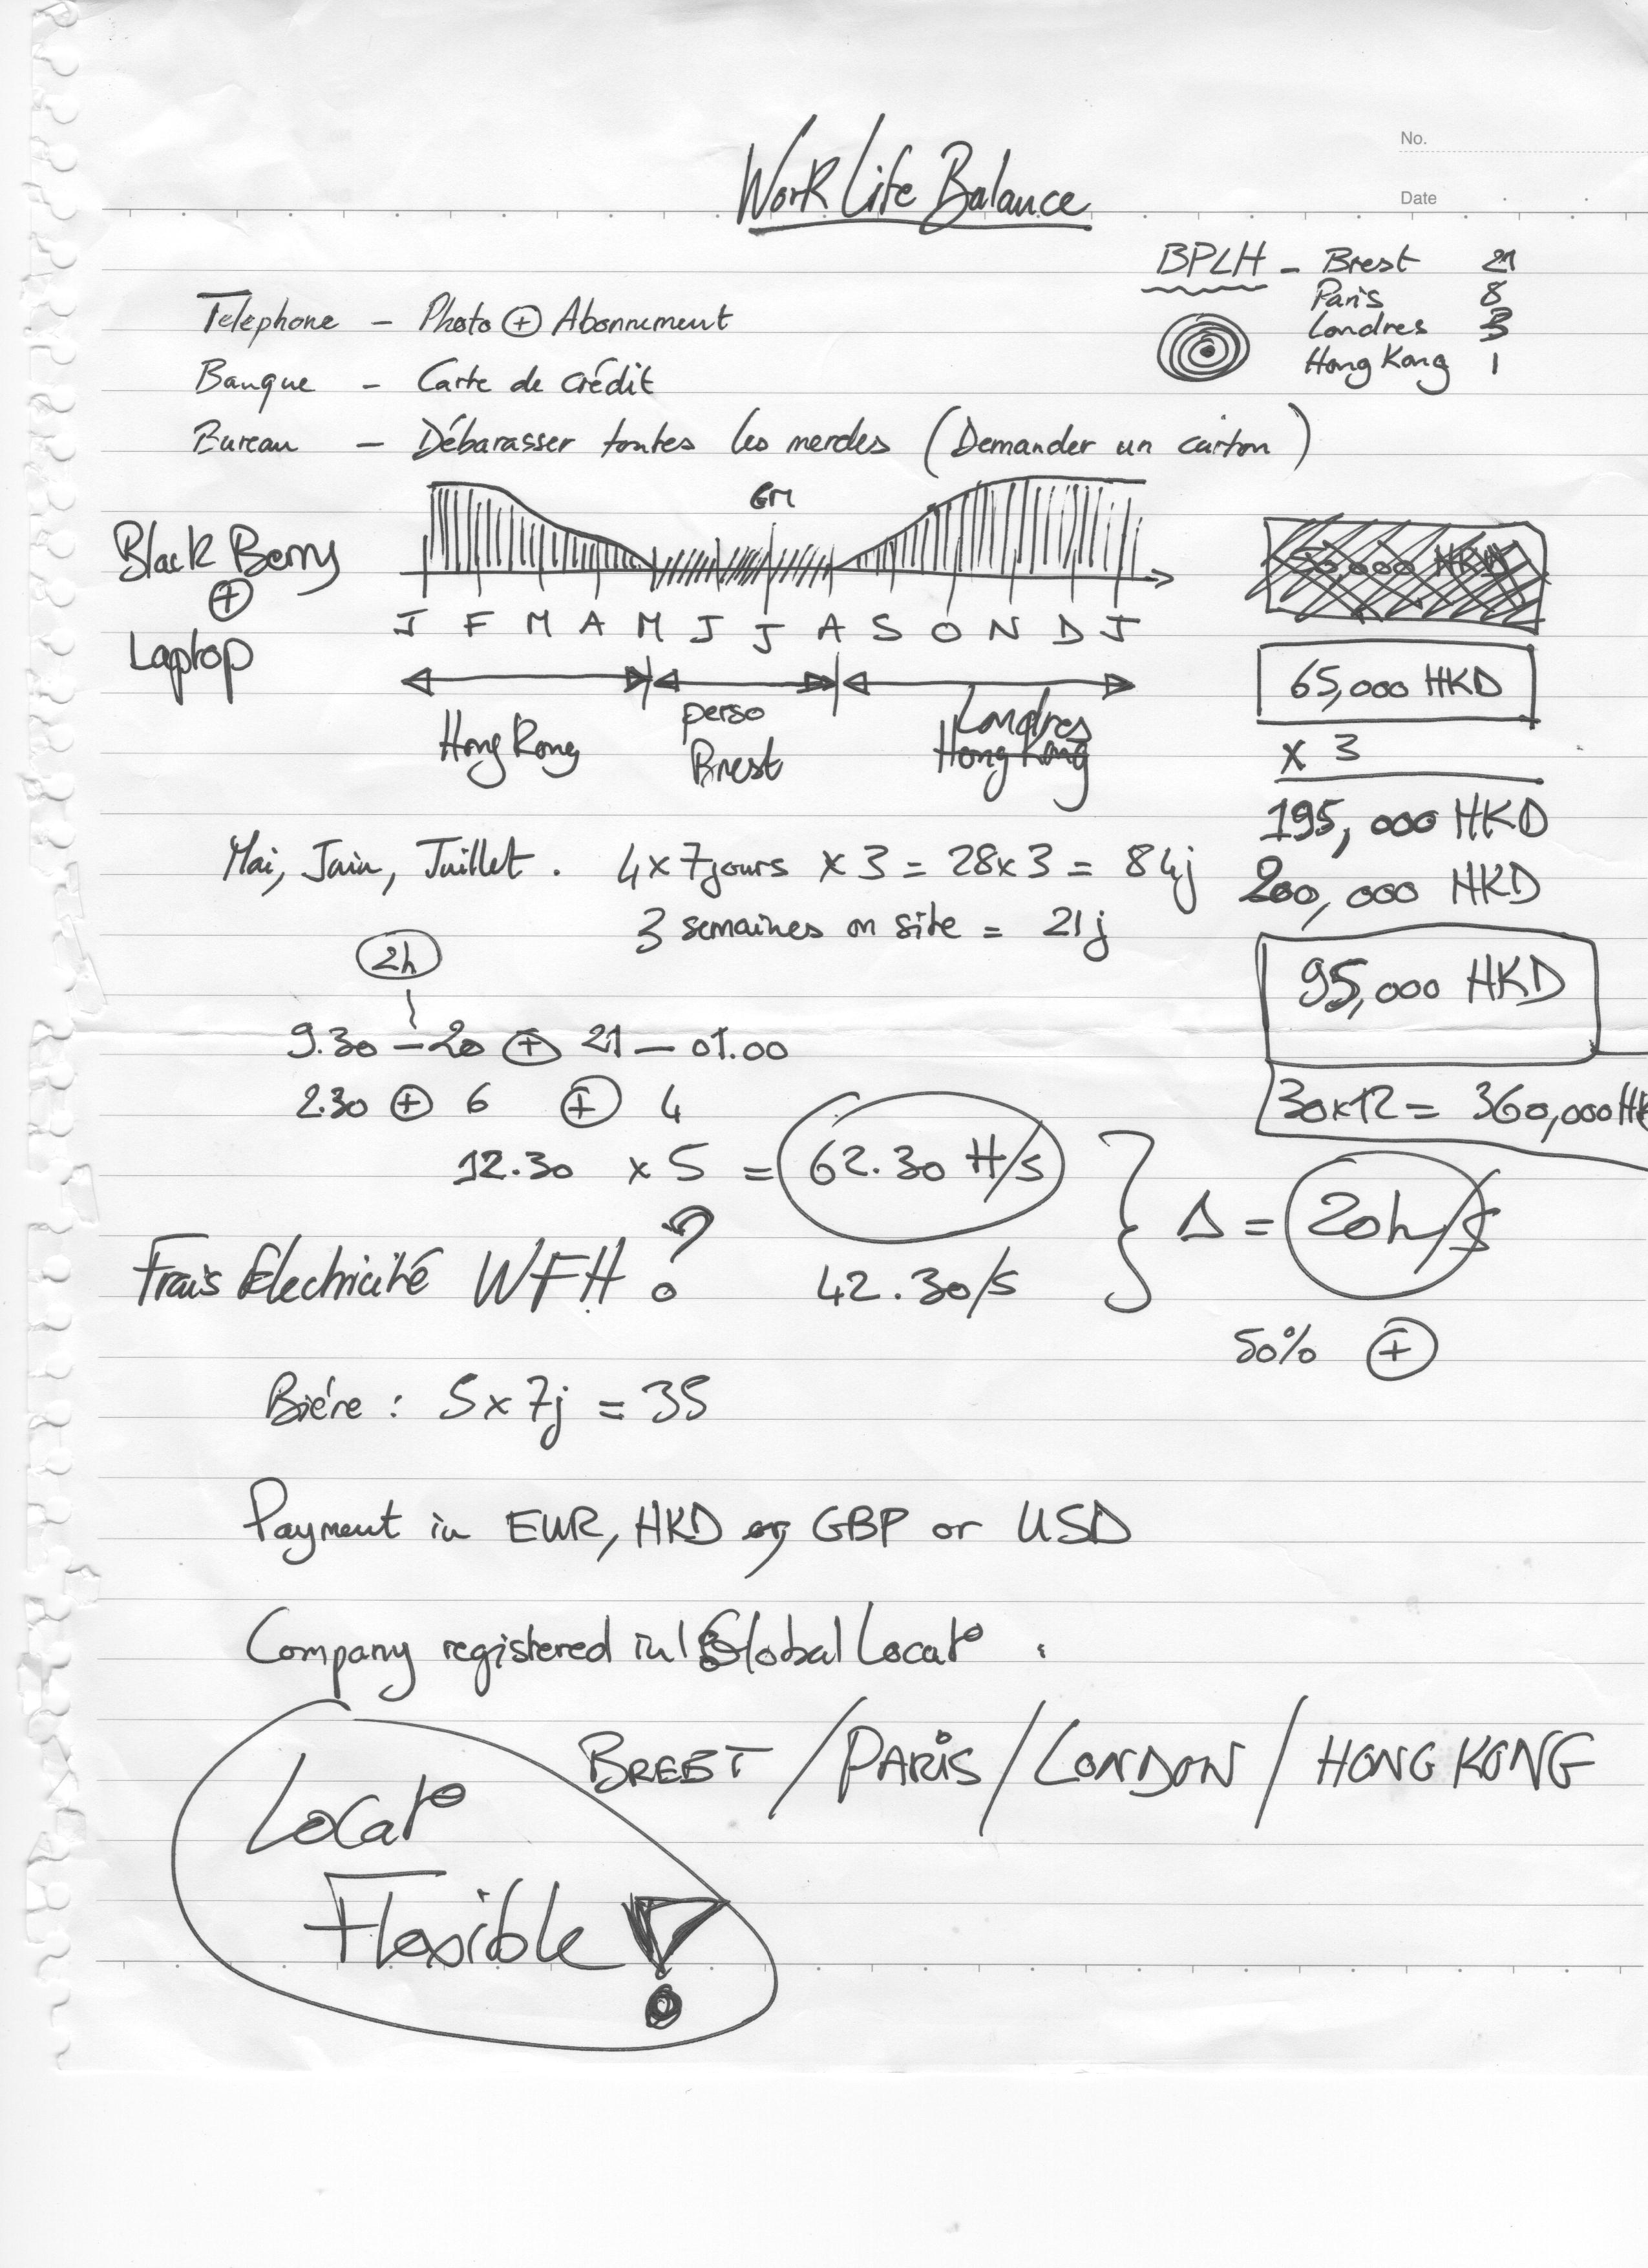
\includegraphics[width=200pts]{007.jpg}

Monthly drift : +280 EUR

\subsection{Assets}

Return on investment?\\

Boat : 27,000 EUR\\
Motor : 6,000 EUR\\
Fields : (4000 EUR)\\
Guitars : 700 EUR\\
Cash : 15,000 EUR\\
Lamp : 350 EUR\\
Guitar folk beige : 350 EUR\\
Mac : 350 EUR\\
Nintendo : 350 EUR\\
Tv samsung : 350 EUR\\
Dvd player : 350 EUR\\

\subsection{Kapital}
To be calculated : Kapital = Assets - Liabilities\\
Leverage?\\

\subsection{Value At Risk}

Monte carlo simulation from bionic turtle/ scilab\\
$\lim_{x \to \infty} \exp(-x) = 0$

\subsection{Sensitivities}
To be calculated : Kapital = Assets - Liabilities


\section{Options}
rating/cost/roii?\\

Bateau plus grand, farming, voiture\\
bateau same, appart, farming voiture\\
maison, farming voiture\\


\section{Projects}

plan/tasks/mgt summ/risks/charge?\\

Elise\\
Climate camp\\
Plijadur\\

\subsection{Tools}
Hudson\\
SVN\\
Clips - ok\\
Scilab - ok\\
Linux\\
MySql\\
Latex - ok\\
Jira\\
Vi - ok\\

\subsection{Deliverables}
\subsection{Document templates}
\subsection{Steps}
Inception\\
Specification\\
Clearchoice\\
External design\\
Internal design\\
Test documentation\\
Release notes\\
Post implementation review\\
Support documentation\\

\subsection{ROI}

\subsection{Budget}

%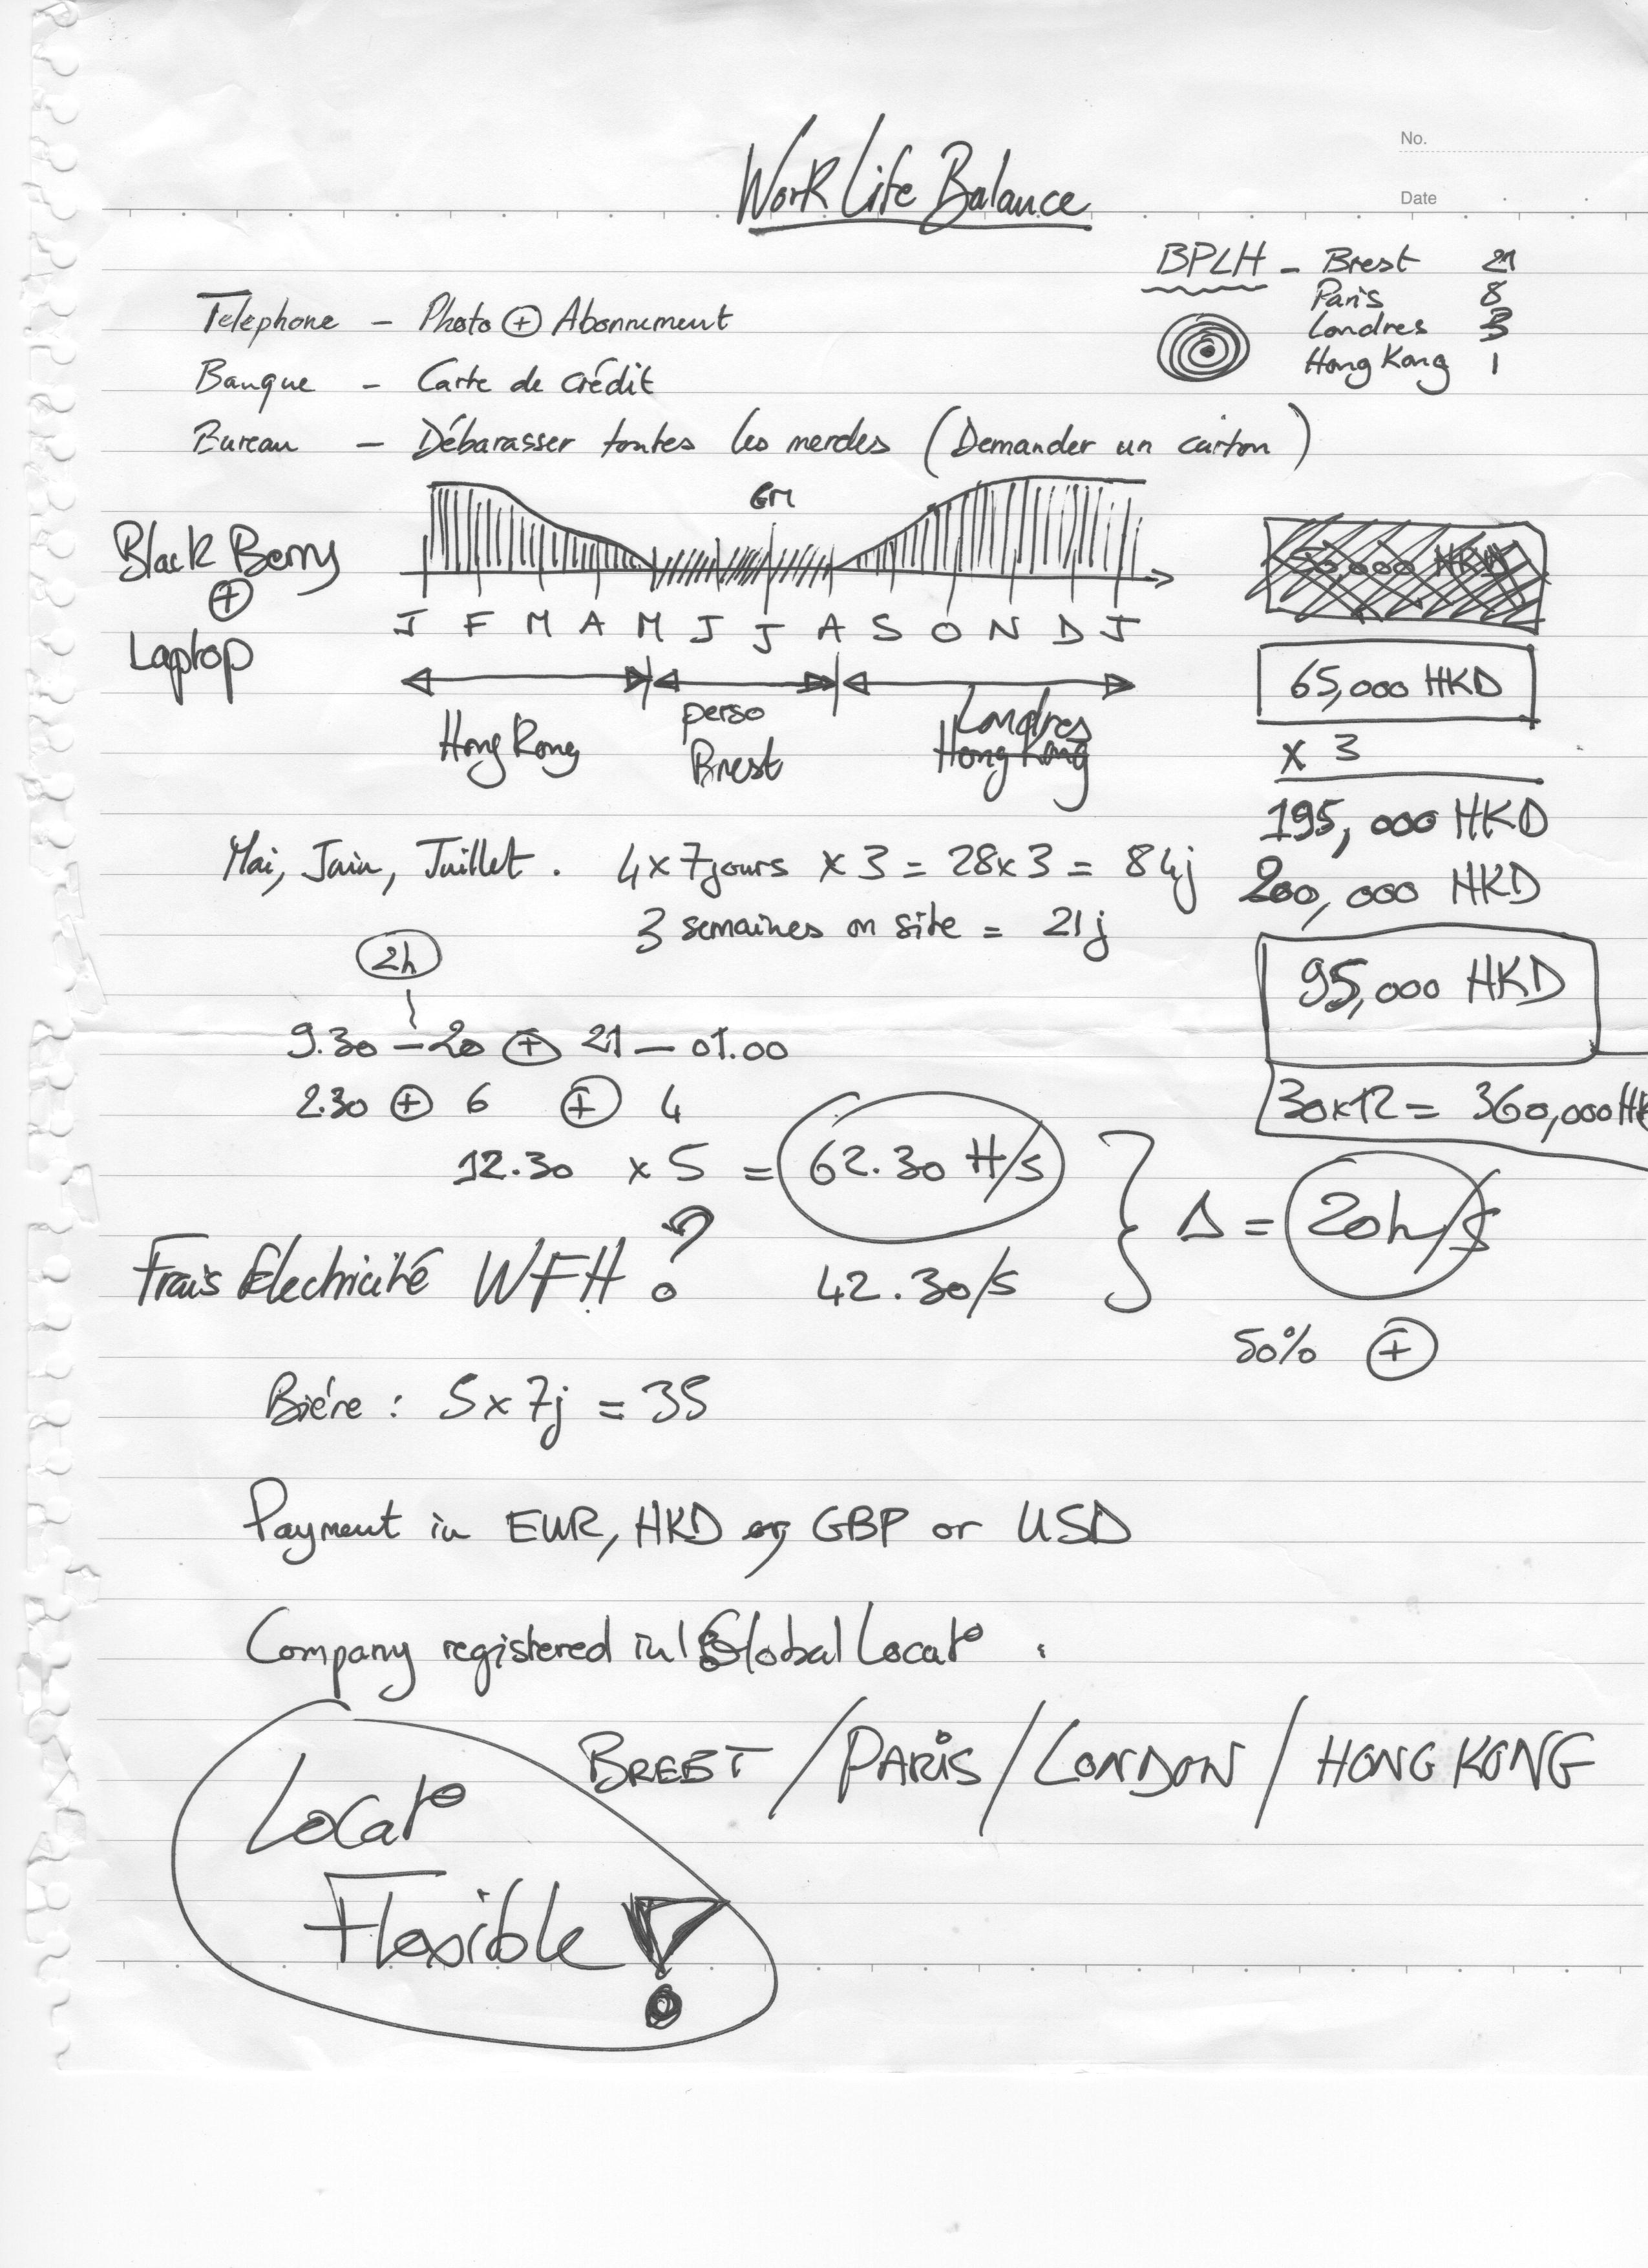
\includegraphics[width=200pts]{007.jpg}
\subsection{Gantt}
%#####################################################################################

\begin{figure}[ftbp]
\begin{center}

\begin{ganttchart}[y unit title=0.4cm,
y unit chart=0.5cm,
vgrid,hgrid, 
title label anchor/.style={below=-1.6ex},
title left shift=.05,
title right shift=-.05,
title height=1,
bar/.style={fill=gray!50},
incomplete/.style={fill=white},
progress label text={},
bar height=0.7,
group right shift=0,
group top shift=.6,
group height=.3,
group peaks={}{}{.2}]{24}
%labels
\gantttitle{Week}{24} \\
\gantttitle{Monday}{4} 
\gantttitle{Tuesday}{4} 
\gantttitle{Wednesday}{4} 
\gantttitle{Thursday}{4} 
\gantttitle{Friday}{4} 
\gantttitle{Saturday}{4} \\
%tasks
\ganttbar{first task}{1}{2} \\
\ganttbar{task 2}{3}{8} \\
\ganttbar{task 3}{9}{10} \\
\ganttbar{task 4}{11}{15} \\
\ganttbar[progress=33]{task 5}{20}{22} \\
\ganttbar{task 6}{18}{19} \\
\ganttbar{task 7}{16}{18} \\
\ganttbar[progress=0]{task 8}{21}{24}

%relations 
\ganttlink{elem0}{elem1} 
\ganttlink{elem0}{elem3} 
\ganttlink{elem1}{elem2} 
\ganttlink{elem3}{elem4} 
\ganttlink{elem1}{elem5} 
\ganttlink{elem3}{elem5} 
\ganttlink{elem2}{elem6} 
\ganttlink{elem3}{elem6} 
\ganttlink{elem5}{elem7} 
\end{ganttchart}
\end{center}
\caption{Gantt Chart}
\end{figure}
%#####################################################################################

\subsection{Resources}
Diagramme en etoile\\

\subsection{Burn down}
Graphique\\
Calcul de vitesse\\
Projection lineaire\\
Specialist tasks\\
Theoretical end\\

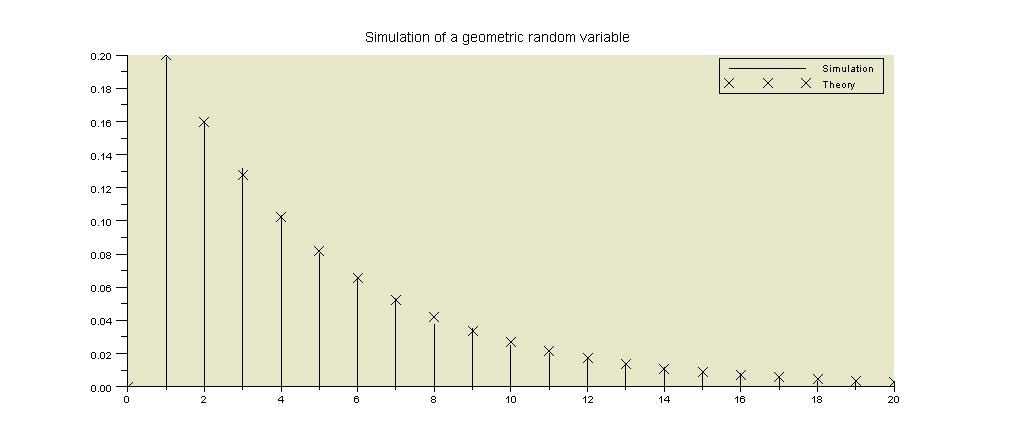
\includegraphics[width=200pts]{Geometric.jpg}

\subsection{Tasks}
List\\
Priorities\\
Cost \\
Dependances\\

\subsection{Risks}
Risk factors\\

\subsection{Meetings}
Team meeting - Daily\\
Steering comittee - Bi weekly\\
Council - Monthly\\

\subsection{Sponsors}
Front office\\
IT\\
Risk management\\
CA\\
HSBC\\

\subsection{Stakeholders}
Front Office : Thibauld Deroux\\
IT : Andrew Jameson\\
Risk management : Axel Brabant\\

\section{Research documents}

\subsection{FX vanilla}
Currency swap\\
FX Spot\\

\subsection{Fx Options}
Simple european pricing\\

\footnote{footnote text}

\subsection{Siv}
Monte Carlo simulation\\

\subsection{Fixed income}
Bond pricing\\

\subsection{IR derivatives}
Amortized swaps\\

\subsection{Equities}
Warrants\\
Vanilla option\\
Stock\\

\subsection{Credit}
CDOs\\
CDSindex\\
CDSbasket\\
Square CDOs

\section{Sports}

\subsection{Football}
Champion de Bretagne\\
Vainqueur de la coupe de Bretagne

\subsection{Sailing}

Crew, date, current, tide, miles, observations
See checklist\\

Brest - Le Fret (secteur ouest force 3-4)\\

Brest - Le Fret - Le Tinduff - Le Fret - Brest (force 6-7 secteur ouest nord ouest) \\
Brest- Camaret - Brest(potes de ja)\\
Brest - Brest\\

Brest - Douarnenez\\
Fred, Etienne, Zaz
Brest - Ouessant\\
Jab, Nico, Elise, Etienne, Fred. 
Brest - Camaret - Brest\\
Fred, Zaz

\subsection{Wakeboard}
Ibiza\\
Rade de Brest\\

\subsection{Canyoning}
Pyrennees\\ 
Corse\\

\subsection{Piloting}
4 lessons with Tim\\

\end{document}
